\section{\sol~ in a Heterogeneous Cluster}
Previously, we discussed the different modules in \sol~ and their major responsibilities. We also formulated the \sol~ scheduling problem and proved that the problem is NP-hard.
In this section, we present the detailed design of \sol~with heuristic container placement and migration algorithms, in a heterogeneous cluster,
which aims to increase resource availability on each worker node and boost the service performance by  approximating the optimal solution of the \sol~ scheduling problem.
To achieve the objectives, \sol~ system consists of three strategies:
%1) Understand the dynamic resource demand of Docker container
1) Identify dominant resource demands of containers;
2) Initial container placement;
3) Migrate a container

\added{[This is good: very clear.]}



\begin{figure*}[ht]
%\hspace*{0.8in}
   \centering
%\vspace{-0.1in}
      \begin{subfigure}[t]{0.24\linewidth}
\centering
      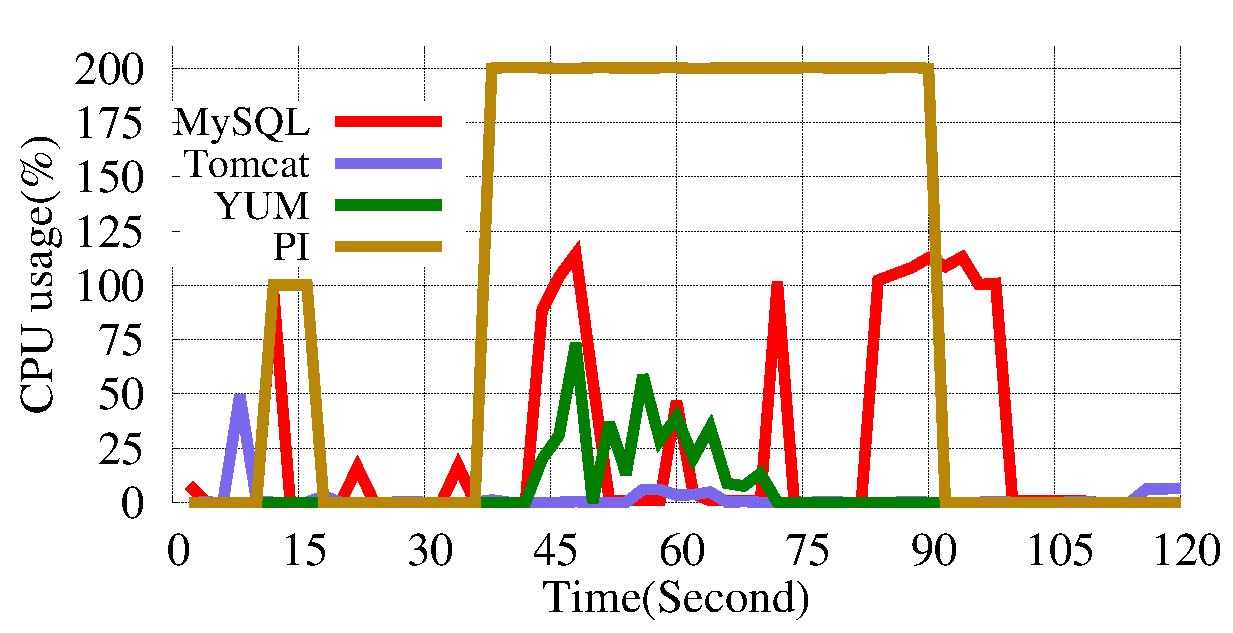
\includegraphics[width=\linewidth]{cpu}
      \vspace{-0.15in}
      \caption{Usage of CPU}
      \label{fig:cpu}
      \end{subfigure} %
      %%%%%%%%%%%%%%%%%%%%%%%%%%%%%%%%
      \begin{subfigure}[t]{0.24\linewidth}
\centering
      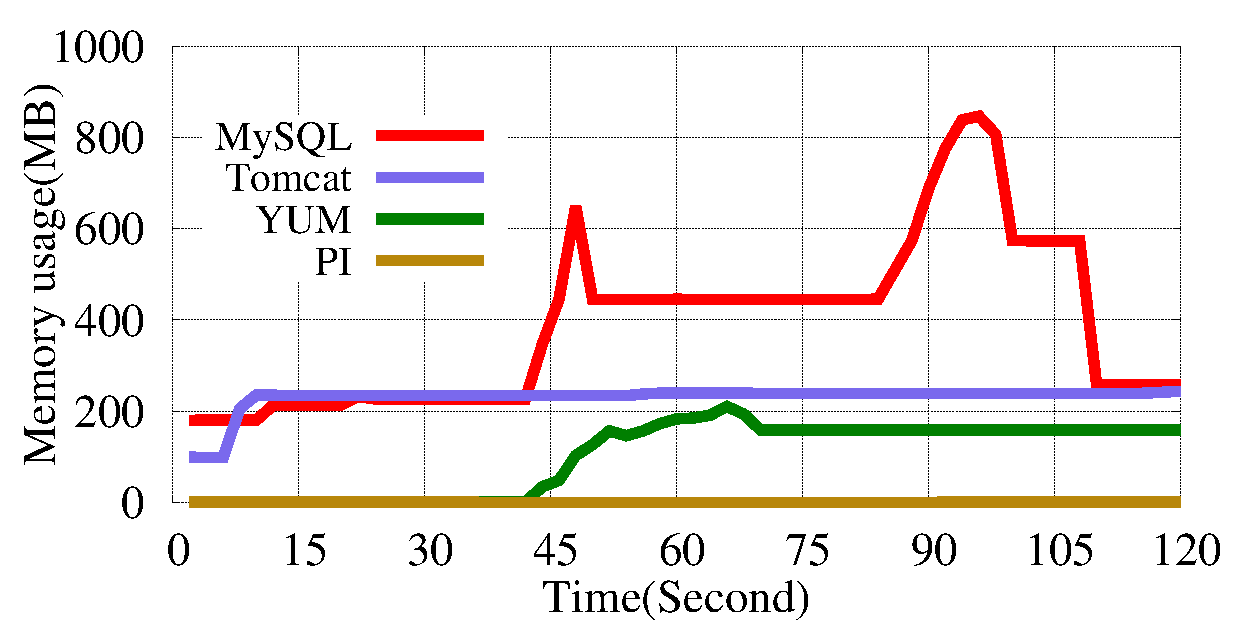
\includegraphics[width=\linewidth]{mem}
      \vspace{-0.15in}
      \caption{Usage of Memory}
      \label{fig:mem}
      \end{subfigure} %
%%%%%%%%%%%%%%%%%%%%%%%%%%%%%%%%%%%%
      \begin{subfigure}[t]{0.24\linewidth}
\centering
      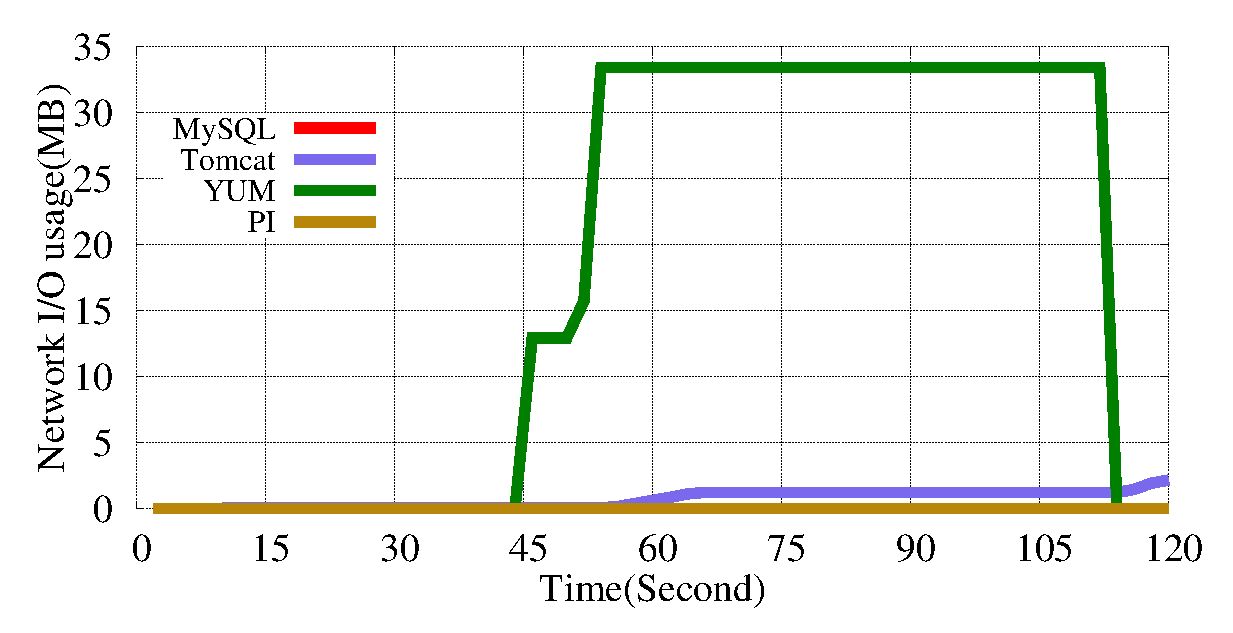
\includegraphics[width=\linewidth]{netio}
      \vspace{-0.15in}
      \caption{Usage of Network I/O}
      \label{fig:netio}
      \end{subfigure} %
      %%%%%%%%%%%%%%%%%%%%%%%%%%%%%%%%
      \begin{subfigure}[t]{0.24\linewidth}
\centering
      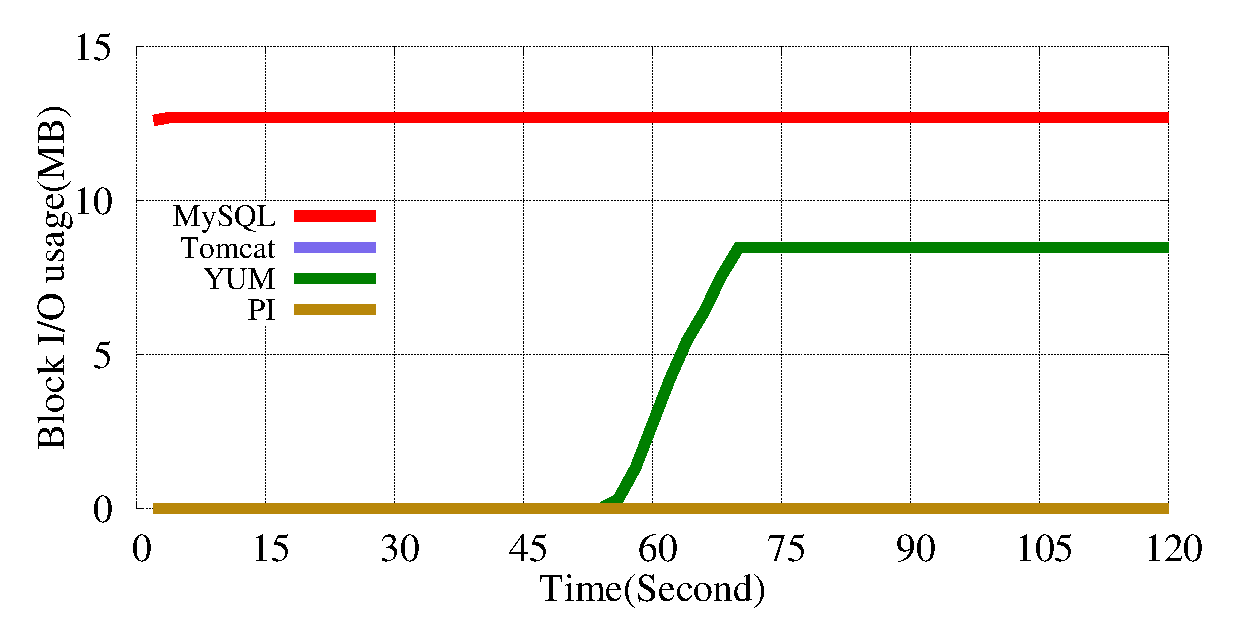
\includegraphics[width=\linewidth]{blockio}
      \vspace{-0.15in}
      \caption{Usage of Block I/O}
      \label{fig:blockio}
      \end{subfigure} %
\caption{Resource demonds under different workloads on four services, MySQL, Tomcat, YUM, PI.}
\label{fig:understand}
\end{figure*}

\subsection{Identify Resource Demands from Containers}
\label{understand}
Before improving the overall resource efficiency, the system needs to understand the dynamic resource demands of various containers.
A container is, usually, focused on providing a specific service, such as web browsing, data sorting, and database querying.
Different algorithms and operations will be applied to the services, which result in diverse resource demands.
As an intuitive example, we conducted the experiments on NSF Cloudlab~\cite{cloudlab} (M400 node hosted by University of Utah).
The containers are initiated by using the following four images and the data is collected through ``docker stats'' command.
\begin{enumerate}
 \item MySQL: the relational database management system. Tested workloads: scan, select, count, join.
 \item Tomcat: provides HTTP web services with Java. Tested workloads: HTTP queries at 10/second and 20/second of a HelloWorld webpage.
 \item YUM: a software package manager that installs, updates, and removes packages. Tested workload: download and install ``vim'' package.
 \item PI: a service to calculate PI. Tested workload: top 3,000 digits with single thread, top 7,500 digits with two threads.
\end{enumerate}
\cref{fig:cpu,fig:mem,fig:netio,fig:blockio} plots the dynamic resource demands under different workloads on the above four Docker containers.
The figures illustrate very diverse usage patterns on four types of resources: CPU, memory, network I/O, and block I/O.
For example, without workload, container PI consumes very limited resources. However, when the jobs arrive at 10th and 38th second, the CPU usage
jumps to 100\% for a single thread job and 200\% for a two-threads job. The usages of the other three types of resources still remain at very low levels.
For MySQL service container, with tested operations, the CPU usage shows a burst when clients submit a request. At time 84, a ``join'' operation that involves
3 tables is submitted, and we can find CPU usage jumps, as well as memory usage. This is because the join operation needs a lot of computation and copies
of tables in memory. Different usage trends are found on YUM and Tomcat services, where YUM uses less CPU and memory, but more network I/O and block I/O to
download and install packages. On the other hand,
Tomcat consumes a very small amount of network I/O and block I/O due to the size of a tested HelloWorld page, but more than 200MB of memory is used to maintain the
service.
To balance the resource usage, it's crucial to place the containers with complementary demands on the same worker.
As shown on the graphs,
there is a dominant resource demand of a service in a given period despite multiple types of resources.

In \sol~, we need to identify the dominant resource demand for each service.
A manager, in the system, can monitor all of the containers' resource usage and group them by their associated service ID.
Suppose the service $s_i \in S$ contains
$m$ running containers that store in a set, $RC_{s_i}$. The resources consumed by $c_i \in RC_{s_i}$ is denoted by a vector,
$R_{c_i}$, where each attribute, $r_i$, in the vector represents a type of resources, such as memory and CPU.
If there are $q$ types of resources in the system, the average resource cost of $s_i$ is a vector, $R_{s_i}$,
$\begin{aligned}
 R_{s_i} & = \sum\nolimits_{c_i \in RC_{s_i}} R_{c_i} \\
         & = <\sum_{c_i \in RC_{s_i}} r_1 / m, \sum_{c_i \in RC_{s_i}} r_2 / m, ..., \sum_{c_i \in RC_{s_i}} r_q / m>
 \end{aligned}
$

On the worker nodes, there is a limited amount of resources in each type.
The resource limit is a vector that contains $q$ attributes, $<l_1, l_2, ..., l_q>$.
The limit of a system, $<L_1, L_2, ..., L_q>$, is obtained by from the sum of vectors from workers.
Therefore,  $R_{s_i}$ can be represented by a percentage of the total resources in the system, for the
$i^{th}$ type, the container cost for $s_i$ in on average is $\sum_{c_i \in RC_{s_i}} r_i / m \div L_i$.
With the analysis, we define the dominant function,
$
  DOM(s_i) = max \{ \sum_{c_i \in RC_{s_i}} r_i / m \div L_i \}
$
Function $DOM(s_i)$ returns the type of a dominant resource demand of service $s_i$ within a given time period.
The value of $DOM(s_i)$ changes along with the
system depending on the running containers for $s_i$ and the current cost of them.


\subsection{Initial Container Placement}
To use a SwarmKit cluster, clients need to execute the command ``docker run'' to start a new container.
Therefore, the first task for the cluster is to choose a worker node to host the container.
As discussed in section~\ref{back}, the default container placement strategy fails to take dynamic
resource contention into consideration. This is because the managers in SwarmKit
do not have a mechanism that can monitor the current available resource.
\sol, on the other hand, addresses the problem by introducing \sol-Heartbeat.
\sol-Heartbeat is an enhanced heartbeat message that not only the states of worker node, but also the
containers' resource usage over a given time window, the usage includes memory, CPU, bandwidth, and block I/O.
On the manager side, the data will be organized into a table that keeps tracking the current available resource
on each worker and its corresponding containers' resource usages.

Running on managers, Algorithm~\ref{alg:initial} assigns a container initialization task to a specific worker.
Firstly, each manager maintains a known service set that records dockers' characteristics, such as the usage of memory, CPU, bandwidth, and block i/o (line 1).
The initial candidate worker are all running workers (line 2).
When a new container starting task arrives, the algorithm applies all filters that the user specified to shrink the candidate work set, $W_{cand}$ (line 3-6).
Then, it checks whether the container belongs to a known service (line 7). If it is, the $S_{dom}$ parameter will be used to store the container's dominant
resource attribute (line 8). In \sol, we consider four types, memory, CPU, bandwidth, and block i/o.
The $W_{cand}$ set will be sorted according to the dominant resource attribute and
return the $W_{id}$ with the highest available resource in $S_{dom}$ type (line 9-10).
If the service cannot be found in $\{KS\}$, $W_{id}$ with the highest available resource on average will be chosen (line 11-13).

\begin{algorithm}[ht]
\begin{algorithmic}[1]
\STATE Maintains a known characteristics service set $\{KS\}$
%and a table that records the current available resource $\{AR\}$;
\STATE $\{W_{cand}\}$ = All running $W_{id}$;
\STATE {\bf Function ContainerPlacement($S_{ID}$)}

\FOR {$w_{id} \in \{W_{cand}\}$}
\IF {$!Filters(w_{id})$}
\STATE Remove $w_{id}$ from $\{W_{cand}\}$
\ENDIF
\ENDFOR

\IF {$S_{ID} \in \{KS\}$}
\STATE $S_{DOM} =  DOM(S_{ID})$
\STATE Sort $W_{cand}$ according to $r_{S_{DOM}}$
\STATE Return $w_{id}$ with highest $r_{S_{DOM}}$

\begin{comment}
  \IF {$S_{dom} = ``M''$}
  \STATE Sort $\{W_{cand}\}$ according to $W_{mem}$
  \STATE Return $W_{id}$ with highest $W_{mem}$

  \ELSIF {$S_{DOM} = ``C''$}
  \STATE Sort $\{W_{cand}\}$ according to $W_{cpu}$
  \STATE Return $W_{id}$ with highest $W_{cpu}$

  \ELSIF {$S_{dom} = ``N''$}
  \STATE Sort $\{W_{cand}\}$ according to $W_{net}$
  \STATE Return $W_{id}$ with highest $W_{net}$

  \ELSIF {$S_{dom} = ``IO''$}
  \STATE Sort $\{W_{cand}\}$ according to $W_{io}$
  \STATE Return $W_{id}$ with highest $W_{io}$
  \ENDIF
\end{comment}

  \ELSE
  \STATE Sort $\sum_{i=0}^{i=q} r_i / m$ for $w_{id} \in W_{cand}$
  \STATE Return $w_{id}$ with highest average available resource

\ENDIF

\end{algorithmic}
\caption{Container Placement on Managers}
\label{alg:initial}
\end{algorithm}



\subsection{Migrating a Container}
In a Swarmkit cluster, resource contention happens on every worker.
The container conitor, which is a module of \sol, runs on each worker to record resource usages of hosting containers.
In addition, the worker keeps tracking available resources on itself. Whenever it finds a draining type of
resources becomes a bottleneck, it sends to managers a \sol~ alert message that contains the bottleneck type and the
most costly container of this type. Upon receiving the \sol~ alert message, the manager needs
to migrate this container to an appropriate worker and kill it on the worker to release the resources.

Algorithm~\ref{alg:migrate} presents the procedure to process an alert message from $w_i$.
It first builds a candidate set $W_{cand}$, which includes all running workers expect $w_i$ that sends the alert (line 1).
Then, the manager extracts the resource type, $r_i$ that causes the bottleneck and finds the corresponding $S_{id}$ for the $C_{id}$ (lines 2-4).
With $W_{cand}$ and $S_{id}$, the algorithm can decide whether this $S_{id}$ is a global service (line 5).
If $S_{id}$ is a global service and it is in the known service set, $\{KS\}$, the algorithm returns $w_{id}$ that is included in $W_{cand}$,
with the highest available $r_{S_{DOM}}$.
On the other hand, it returns $w_{id}$ with the highest available $r_i$ if $S_{id}$ is not in $\{KS\}$ and $S_{DOM}$ on unknown (lines 6-12).
When $S_{id}$ is not a global service, we want to increase the reliability of $S_{id}$ by placing its containers to different workers as much as possible.
In this situation, we have a similar process expect a different $W_{cand}$, where $W_{cand}$  contains all running
workers that do not hosting any containers for $S_{id}$ (lines 13 - 23).



\begin{algorithm}[ht]
\begin{algorithmic}[1]

\STATE $\{W_{cand}\}$ = All running workers expect $w_i$;
\STATE {\bf Function ReceiveAlertMsg($C_{id}$)}
\STATE Extract the bottleneck type $r_i$
\STATE Find corresponding $S_{id}$ for $C_{id}$


\IF {$\forall w_{id} \in W_{cand} \rightarrow S_{id} \in w_{id}$}

  \IF {$S_{id} \in \{KS\}$}
  \STATE $S_{DOM} = DOM(S_{id})$

%  \IF {$S_{DOM} \neq r_i$}
%  \STATE Return Restart the container on $w_i$
%  \ENDIF

\STATE Sort $W_{cand}$ according to $r_{S_{DOM}}$
\STATE Return $w_{id}$ with highest $r_{S_{DOM}}$

\ELSE
%\STATE $\forall w_{id} \in W_{cand}$, Remove $w_{id}$ from $W_{cand}$
\STATE Sort $W_{cand}$ according to $r_i$
\STATE Return $w_{id}$ with highest $r_i$

\ENDIF

  \ELSE
  \FOR {$ w_{id} \in W_{cand}$}
  \IF {$S_{id} \in w_{id}$}
  \STATE Remove $w_{id}$ from $W_{cand}$
  \ENDIF
  \ENDFOR
%  \STATE Sort $W_{cand}$ according to $r_i$
%  \STATE Return $W_{id}$ with highest available resource type $r_i$

\IF {$S_{id} \in \{KS\}$}
  \STATE $S_{DOM} = DOM(S_{id})$

%  \IF {$S_{DOM} \neq r_i$}
%  \STATE Return Restart the container on $w_i$
%  \ENDIF

\STATE Sort $W_{cand}$ according to $r_{S_{DOM}}$
\STATE Return $w_{id}$ with highest $r_{S_{DOM}}$

\ELSE
%\STATE $\forall w_{id} \in W_{cand}$, Remove $w_{id}$ from $W_{cand}$
\STATE Sort $W_{cand}$ according to $r_i$
\STATE Return $w_{id}$ with highest $r_i$

\ENDIF

\ENDIF



\end{algorithmic}
\caption{Process \sol~ Alert Message from $w_i$}
\label{alg:migrate}
\end{algorithm}
